\documentclass{standalone}
\usepackage{tikz}
\begin{document}
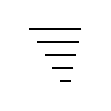
\begin{tikzpicture}[xscale=-.4, yscale=-1]
  \pgfmathsetmacro{\nmax}{5}
  \pgfmathsetmacro{\oneup}{\nmax+1}

  \pgfmathsetmacro{\nstart}{1}
  \pgfmathsetmacro{\nsecond}{\nstart+1}

  \pgfmathsetmacro{\offset}{0}
  \pgfmathsetmacro{\dx}{(\nmax-\nstart)/\oneup}

  \foreach \n in {\nstart,\nsecond,...,\nmax}{
    \pgfmathsetmacro{\offset}{\offset + \n/12}

    \pgfmathsetmacro{\dx}{\n/\oneup}

    \pgfmathsetmacro{\xstart}{1 - \dx + \offset}
    \pgfmathsetmacro{\xend}{1 + \dx + \offset}
    \pgfmathsetmacro{\y}{1-\n/\oneup}
    \draw[line width=.8pt] (\xstart, \y) -- (\xend, \y);
  }
\end{tikzpicture}

\end{document}
